{\color{gray}\hrule}
\section{What makes a review good?}

\subsection{Up votes And Funny Votes}

\begin{figure}[H]
    \centering
    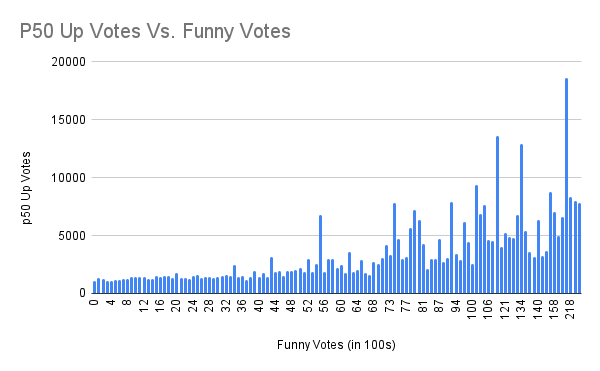
\includegraphics[width=0.8\linewidth]{visuals/P50 Up Votes Vs. Funny Votes (2)}
    \caption{Top 10000 up voted reviews vs their funny votes in 100s}
    \label{fig:p50 Up Votes Vs. Funny Votes(100s)}
\end{figure}

 I my hypothesis by plotting the top 10,000 most voted reviews against the number of funny votes it receives in figure 1. The graph depicts the weak positive correlation between funny votes and up votes. This disproved my hypothesis and shows that humor generally played a smaller role. Note, the higher variation at the upper ends is a result of the smaller sample of highly rated funny reviews.

\subsection{User role in reviews?}
Given that humor plays a small role in a good review, I hypothesized that Steam users favored more knowledgeable and informative reviews. To define the knowledge of a user, it is the combination of the number of hours at playtime, the number of games the user own, and the number of reviews a user has written. 

\begin{figure}[H]
    \centering{}
    \caption{Avg Up Votes Vs. User Total Reviews}

    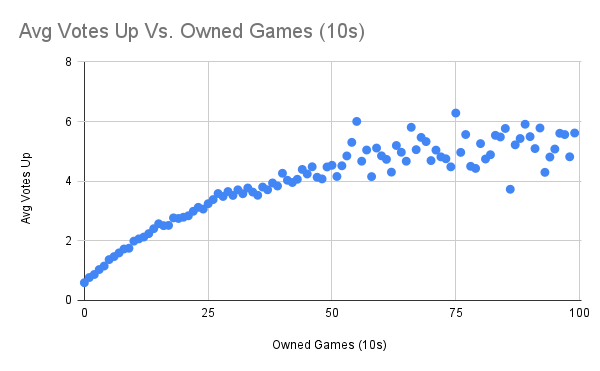
\includegraphics[width=0.8\linewidth]{visuals/Avg Votes Up Vs. Owned Games (10s)}
    \label{fig:Average Up Votes Vs. Num Games Owned (10s)}
\end{figure}

\begin{figure}[H]
    \centering
    \subfloat{
        \begin{minipage}{0.48\textwidth}  % Adjust width as needed
            \centering
            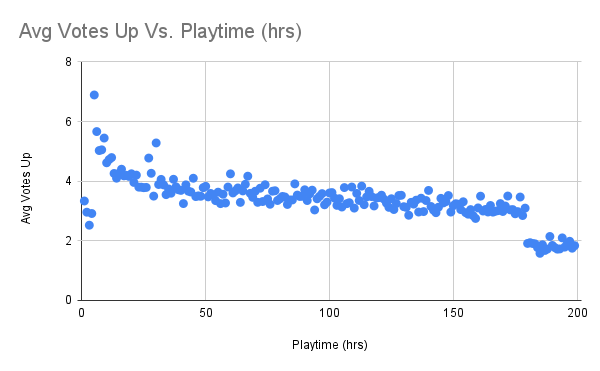
\includegraphics[width=1\linewidth]{visuals/Avg Votes Up Vs. Playtime (hrs)}
            \label{fig:Avg Up Votes VS. Playtime (1000hrs)}
        \end{minipage}
    }
    \subfloat{
        \begin{minipage}{0.48\textwidth}  % Adjust width as needed
            \centering
            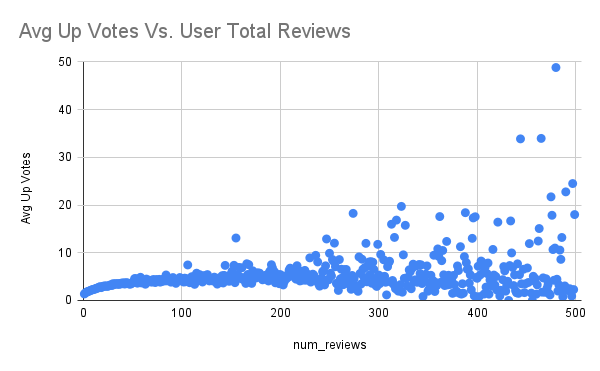
\includegraphics[width=1\linewidth]{visuals/Avg Up Votes Vs. User Total Reviews}
            \label{fig:Avg Up Votes VS. Playtime (1000hrs)}
        \end{minipage}
    }
    \caption{User Data Vs. Avg Up Votes}
\end{figure}

From the above, the number of games a user owned has a linear relationship to the number of up votes. This suggest that users with more owned games make better reviews than those with fewer games owned. This aligns with my hypothesis that users value experience in a review. On the other hand, good reviews peak at 10 hours of playtime. Interestingly after 170 hours, the up votes takes another dip. I underestimated how much users viewed playtime as a sign of bias. On the other hand, the number of reviews a user has made seems to have a positive effect on up votes, but this stops at around 100 reviews. My hypothesis was partial correct, but I misunderstood playtime and overestimated the role of humor. 
